\chapter{Introduzione ai gruppi}

Lo scopo di questo capitolo è quello di introdurre il concetto di gruppo, mostrando alcuni esempi espliciti di gruppo, introducendone gli assiomi. La teoria dei gruppi, nonostante la sua applicazione alla Fisica sia piuttosto moderna, riveste un ruolo fondamentale, in quanto rappresenta il linguaggio naturale delle simmetrie dei sistemi fisici, classici e non, che incontriamo tutti i giorni.

\section{Assiomi di gruppo e teoria degli insiemi}

Se volessimo definire formalmente un gruppo, potremmo dare la seguente definizione

\begin{definition}[gruppo]
	Sia $G$ un insieme e sia $\cdot: G \times G \to G$ un'operazione, che chiameremo \emph{prodotto} che possiede le seguenti proprietà:
	\begin{enumerate}
		\item $\forall g_1, g_2 \in G, \exists g_3 \in G : g_1 \cdot g_2 = g_3$;
		\item $\forall g_1, g_2, g_3 \in G, g_1 \cdot (g_2 \cdot g_3) = (g_1 \cdot g_2) \cdot g_3$ (proprietà associativa);
		\item $\exists e \in G: \forall g \in G, e \cdot g = g$ (esistenza dell'elemento neutro);
		\item $\forall g \in G, \exists g^{-1} \in G: g^{-1} \cdot g = e$ (esistenza dell'elemento inverso);
	\end{enumerate}
\end{definition}

Da questi assiomi discendono le seguenti proprietà
\begin{prop}
	Se $(G, \cdot)$ è un gruppo, allora
	\begin{equation}
	\forall g \in G, g^{-1} \cdot g = g \cdot g^{-1} = e. 
	\end{equation}
\end{prop}
\begin{proof}
	Preso $g \in G$, sappiamo che $g^{-1} \cdot g = e$, in virtù dell'assioma $\circled{3}$, dunque sappiamo che, in virtù dell'assioma $\circled{4}$, possiamo moltiplicare a sinistra entrambi i lati per
	l'elemento inverso di $g^{-1}$, da cui 
	\begin{align}
	&g^{-1} \cdot g = e \implies (g^{-1})^{-1} \cdot g^{-1} \cdot g = (g^{-1})^{-1} \cdot e
	\end{align}
	e moltiplichiamo a destra entrambi i lati per $g^{-1}$ così da ottenere l'espressione di cui stiamo cercando il valore, ottenendo che
	\begin{align}
	&(g^{-1})^{-1} \cdot g^{-1} \cdot g \cdot g^{-1} = (g^{-1})^{-1} \cdot e \cdot g^{-1}\\
	\end{align}
	e a questo punto usiamo l'assioma $\circled{3}$ e l'assioma $\circled{4}$ per concludere che
	\begin{align}
	&e \cdot g \cdot g^{-1} = e \implies g \cdot g^{-1} = e.
	\end{align}
	La tesi segue dall'arbitrarietà di $g$.
\end{proof}


\begin{prop}
	Se $(G, \cdot)$ è un gruppo, allora
	\begin{equation}
		\forall g \in G, g \cdot e = e \cdot g = g. 
	\end{equation}
\end{prop}
\begin{proof}
	Partiamo dall'uguaglianza (garantita dagli assiomi)
	\begin{equation}
		e \cdot g = g,
	\end{equation}
	da cui usando l'assioma $\circled{4}$, moltiplicando entrambi i lati ``a sinistra" per $g^{-1}$ si consegue che
	\begin{equation}
		g^{-1} \cdot e \cdot g = g^{-1} \cdot g,
	\end{equation}
	e sempre usando l'assioma $\circled{4}$, unita alla proposizione appena mostrata sopra, si ottiene che
	\begin{equation}
		g^{-1} \cdot e \cdot e = e \cdot g^{-1},
	\end{equation}
	da cui si ottiene, usando l'assioma $\circled{3}$, che
	\begin{equation}
		g^{-1} \cdot e = g^{-1}.
	\end{equation}
	La tesi segue dall'arbitrarietà di $g$ e, conseguentemente, dall'arbitrarietà di $g^{-1}$
\end{proof}

\begin{prop}
	Sia $(G, \cdot)$ un gruppo, allora abbiamo che l'elemento neutro è unico.
\end{prop}

\begin{proof}
	Se per assurdo avessimo che $\exists e, e' \in G, e \neq e'$ tali che
	\begin{align}
		\forall g \in G, \begin{cases*}
			e \cdot g = g \\
			e' \cdot g = g
		\end{cases*}
	\end{align}
	allora si ha che
	\begin{equation}
		e \cdot e' = e,
	\end{equation}
	ma per la proposizione precedente abbiamo che
	\begin{equation}
		e = e \cdot e' = e' \cdot e = e'.
	\end{equation}
	Segue quindi che $e = e'$, il che è un assurdo.
\end{proof}

\begin{prop}
	Sia $(G, \cdot)$ un gruppo, allora
	\begin{equation}
		\forall g \in G, \exists! g^{-1} \in G : g^{-1} \cdot g = e.
	\end{equation}
\end{prop}
\begin{proof}
	Se per assurdo avessimo che $\exists g^{-1}, (g^{-1})' \in G, g^{-1} \neq (g^{-1})'$, con $g^{-1} \cdot g = e$ e $(g^{-1})' \cdot g = e$, allora si ha che
	\begin{equation}
		g^{-1} \cdot g = e = (g^{-1})' \cdot g \implies g^{-1} \cdot g \cdot g^{-1} = (g^{-1})' \cdot g \cdot g^{-1} \implies g^{-1} = (g^{-1})'.
	\end{equation}
\end{proof}

Siccome i gruppi sono degli insiemi, è chiaramente naturale dover esprimere alcuni risultati dei gruppi usando il linguaggio insiemistico: rivediamo, quindi, quali sono gli assiomi
principali che governano la teoria degli insiemi che useremo:

\begin{enumerate}
	\item se un elemento $g$ appartiene ad un insieme $M$, scriveremo che
	\begin{equation}
		g \in M,
	\end{equation}
	se invece consideriamo un insieme di elementi scriveremo che
	\begin{equation}
		\{ g_i \} \in M,
	\end{equation}
	dove a priori $i$ potrebbe essere anche un parametro continuo.
	\item se $M, N$ sono insiemi, allora è ben definito $M \cup N$ e diremo che
	\begin{equation}
		g \in M \cup N \iff g \in M \vee g \in N,
	\end{equation}
	\item se $M, N$ sono insiemi, allora è ben definito $M \cap N$ e diremo che
	\begin{equation}
		g \in M \cap N \iff g \in M \wedge g \in N,
	\end{equation}
	\item se $M, N$ sono insiemi, allora è ben definito $M \backslash N$ e diremo che
	\begin{equation}
		g \in M \backslash N \iff g \in M \vee g \not\in N.
	\end{equation}
\end{enumerate}

Da questi assiomi, possiamo anche dare la definizione di \emph{sottoinsieme}
\begin{definition}[sottoinsieme]
	Siano $M, N$ due insiemi, diremo che $N$ è un sottoinsieme di $M$ se
	\begin{equation}
		\forall a, a \in N \implies a \in M,
	\end{equation}
	e scriveremo che $N \subseteq M$.
\end{definition}

Inoltre, un concetto che utilizzeremo spesso è quello di \emph{relazione d'equivalenza}, di cui riportiamo la definizione formale

\begin{definition}[relazione d'equivalenza]
	Sia $M$ un insieme e sia $\sim \subseteq M \times M$, diremo che $\sim$ è una relazione d'equivalenza se gode delle seguenti proprietà
	\begin{enumerate}[label=\protect\circled{\arabic*}]
		\item \textbf{riflessività}: $a \sim a$ (o più formalmente $(a, a) \in \sim$);
		\item \textbf{simmetricità}: $a \sim b \implies b \sim a$ (o più formalmente $(a, b) \in \sim \implies (b, a) \in \sim$);
		\item \textbf{transitività}: $a \sim b, b \sim c \implies a \sim c$ (o più formalmente $(a, b), (b, c) \in \sim \implies (a, c) \in \sim$).
	\end{enumerate}
\end{definition}

Possiamo a questo punto definire le funzioni: non forniremo una costruzione insiemistica delle funzioni, anche se ciò potrebbe essere fatto. Considereremo le funzioni fra insiemi, dunque,
come delle semplici scatole magiche che prendono un elemento di un insieme e restituiscono un solo elemento di un altro insieme.

\begin{definition}[mappe]
	Diremo che una mappa è una relazione $f$ fra due insiemi $M, N$ tale per cui
	\begin{equation}
		\forall g, g \in M \implies y=f(g) \in M,
	\end{equation}
	e diremo che $y$ è l'immagine di $g$ tramite $f$.
\end{definition}

Da questa definizione possiamo, ovviamente, dare le usuali definizioni di mappa iniettiva e surgettiva,

\begin{definition}[mappa iniettiva]
	Siano $M, N$ due insiemi, diremo che la mappa $f: M \to N$ è iniettiva se
	\begin{equation}
		\forall g_1, g_2 \in M, g_1 \neq g_2 \implies f(g_1) \neq f(g_2).
	\end{equation}
\end{definition}

\begin{definition}[mappa surgettiva]
	Siano $M, N$ due insiemi, diremo che la mappa $f: M \to N$ è suriettiva se
	\begin{equation}
		\forall b \in N, \exists a \in M : a \stackrel{f}{\mapsto} b. 
	\end{equation}
\end{definition}

e, chiaramente, la definizione di mappa ``1 a 1" o bigettiva,

\begin{definition}[mappa bigettiva]
	Siano $M, N$ due insiemi, diremo che la mappa $f: M \to N$ è bigettiva se è iniettiva e suriettiva, ovvero
	\begin{equation}
		\forall b \in N, \exists! a \in M : f(a) = b.
	\end{equation}
\end{definition}
Ricordiamo, ovviamente, che esistono mappe iniettive ma non surgettive, mappe surgettive ma non iniettive e mappe né surgettive né iniettive: per esempio si può considerare 
\begin{itemize}
	\item $f: \mathbb{R} \to \mathbb{R}$ con $f(x) = x$, che risulta essere bigettiva;
	\item $f: \mathbb{R} \to \mathbb{R}$ con $f(x) = x^3$, che risulta essere bigettiva;
	\item $f: \mathbb{R} \to \mathbb{R}$ con $f(x) = x^2$, che non è né iniettiva né surgettiva;
	\item $f: \mathbb{R} \to \mathbb{R}$ con $f(x) = x(x^2 - 1)$, che non è iniettiva ma è surgettiva;
	\item $f: \mathbb{R} \to \mathbb{R}$ con $f(x) = e^x$, che è iniettiva ma non surgettiva;
	\item $x^2 + y^2 = 1$ non è una mappa, infatti se $x \in (-1, 1) \implies y \not\in \mathbb{R}$ (abbiamo due soluzioni, quindi due elementi possibili, dunque non è una mappa).
\end{itemize}

Un tipo di mappa molto importante è quella \emph{di rivestimento}, di cui riportiamo una breve definizione visto che la useremo
\begin{definition}
	Siano $M, N$ due varietà della stessa dimensione, allora se $x \in M, y \in N$ e $x \mapsto y(x)$ con
	\begin{enumerate}[label=\protect\circled{\arabic*}]
		\item $\forall y \in N, \text{det}\left( \frac{\partial y_i}{\partial x_j} \right) \neq 0$;
		\item $\forall y \in N$ ha un insieme numerabile o finito di controimmagini;
		\item $\forall y \in N, \exists U_i$ intorno di $y$ in $N$ tale che la sua controimmagine è unione disgiunta di intorni $V_{ik}$ con $k = 1, 2, \ldots$, ovvero
		\begin{equation}
			f^{-1}(U_i) = \bigcup_{k=1} V_{ik},
		\end{equation}
		e il \# di intorni è detto \# di fogli di $f$: per esplicitare ciò, diremo che $M \stackrel{f}{\mapsto} N$ è a \# fogli.
	\end{enumerate}
\end{definition}

\begin{figure}[htbp]
	\centering
	\begin{tikzpicture}[>=Stealth, scale=1.3]
		
		% --- SPAZIO BASE X (in basso) ---
		% Il manifold base
		\draw[fill=gray!10, thick] (0,-3) ellipse (3.5cm and 1cm);
		\node[font=\large] at (-4, -3) {$N$};
		
		% Il punto y
		\coordinate (y) at (0,-3);
		
		% L'intorno U banalizzante
		% Usiamo un'ellisse tratteggiata per l'aperto
		\draw[dashed, fill=blue!20, opacity=0.7, thick] (y) ellipse (1cm and 0.5cm);
		\node[blue!80!black, font=\bfseries] at (1.3, -3) {$U$};
		\filldraw (y) circle (1.5pt) node[below, font=\small] {$y$};
		
		
		% --- SPAZIO TOTALE \tilde{X} (in alto) ---
		% Disegniamo una grande ellisse che rappresenta una porzione di \tilde{X}
		\draw[fill=gray!5, thick] (0, 2.5) ellipse (4cm and 1.8cm);
		\node[font=\large] at (-4.5, 2.5) {$M$};
		\node[font=\small, gray] at (0, 3.7) {Controimmagine $p^{-1}(U) = \bigsqcup V_i$};
		
		% --- LE "PALLE" V_i (Controimmagini) ---
		% Definiamo i centri delle tre palle
		\coordinate (yt1) at (-2.2, 2.2);
		\coordinate (yt2) at (0, 2.8);
		\coordinate (yt3) at (2.2, 2.2);
		
		% Palla V_1
		\draw[dashed, fill=red!20, opacity=0.7, thick] (yt1) circle (0.7cm);
		\filldraw (yt1) circle (1.5pt) node[above, font=\small] {$x_1$};
		\node[red!80!black, font=\bfseries] at ($(yt1)+(-0.2,-1)$) {$V_1$};
		
		% Palla V_2 (quella centrale)
		\draw[dashed, fill=red!20, opacity=0.7, thick] (yt2) circle (0.7cm);
		\filldraw (yt2) circle (1.5pt) node[above, font=\small] {$x_2$};
		\node[red!80!black, font=\bfseries] at ($(yt2)+(-0.2,-1)$) {$V_2$};
		
		% Palla V_3
		\draw[dashed, fill=red!20, opacity=0.7, thick] (yt3) circle (0.7cm);
		\filldraw (yt3) circle (1.5pt) node[above, font=\small] {$x_3$};
		\node[red!80!black, font=\bfseries] at ($(yt3)+(-0.25,-1)$) {$V_3$};
		
		
		% --- MAPPE DI PROIEZIONE p ---
		% Frecce grosse che mostrano che l'intero insieme V_i va in U
		
		% Freccia da V1 a U
		\draw[->, ultra thick, opacity=0.5, red!60!blue, shorten >= 5pt, shorten <= 5pt] 
		($(yt1)+(0,-0.7)$) to[out=-80, in=160] ($(y)+(-0.8, 0.3)$);
		
		% Freccia da V2 a U (centrale)
		\draw[->, ultra thick, opacity=0.5, red!60!blue, shorten >= 5pt, shorten <= 5pt] 
		($(yt2)+(0,-0.7)$) -- ($(y)+(0, 0.5)$);
		
		% Freccia da V3 a U
		\draw[->, ultra thick, opacity=0.5, red!60!blue, shorten >= 5pt, shorten <= 5pt] 
		($(yt3)+(0,-0.7)$) to[out=-100, in=20] ($(y)+(0.8, 0.3)$);
		
		% Etichetta della mappa
		\node[font=\large, right] at (2.5, -0.5) {$p$};
		
	\end{tikzpicture}
	\caption{Sketch grafico della \protect\circled{3} richiesta dalla definizione di mappa di rivestimento. In questo caso, se la mappa $p$ soddisfa la \protect\circled{1}, \protect\circled{2} allora sarebbe una mappa a $3$ fogli.}
\end{figure}

Vediamo qualche esempio di mappa di rivestimento: l'esempio più semplice è quello rappresentato dalla funzione $w = f(z) = z^n$ con $f: S^1 \to S^1$ che mappa il cerchio unitario
nel cerchio unitario. E' chiaro che preso $w \in S^1$, allora esistono $n$ soluzioni all'equazione $z^n = w$, dunque diremo che è una mappa a $n$ fogli.
\begin{figure}[htbp]
    \centering
    \begin{tikzpicture}[>=Stealth, scale=1.3]

        % --- SPAZIO BASE S^1 (sotto) ---
        \begin{scope}[shift={(0,-3)}]
            % Intera circonferenza base (grigio chiaro per indicare la varietà totale)
            \draw[thick, gray!50] (0,0) ellipse (2.5 and 1);
            \node[font=\large] at (-3.2, 0) {$S^1$};
            
            % Intorno banalizzante U (arco blu) - es. da -30° a 30°
            \draw[ultra thick, blue!80] ({2.5*cos(-30)}, {1*sin(-30)}) arc (-30:30:2.5 and 1);
            
            % Punto y sulla base (usiamo il punto 1)
            \filldraw (2.5, 0) circle (1.5pt) node[right, font=\small, black] {$1$};
            \node[blue!80!black, font=\bfseries] at (2.8, 0.5) {$U$};
        \end{scope}

        % --- SPAZIO TOTALE S^1 (sopra) ---
        \begin{scope}[shift={(0,2)}]
            % Intera circonferenza di rivestimento
            \draw[thick, gray!50] (0,0) ellipse (2.5 and 1);
            \node[font=\large] at (-3.2, 0) {$S^1$};
            
            % Preimmagine V1 (attorno a 0°) - da -10° a 10°
            % Essendo z^3, l'arco sopra è un terzo di quello sotto
            \draw[ultra thick, red!80] ({2.5*cos(-10)}, {1*sin(-10)}) arc (-10:10:2.5 and 1);
            \filldraw (2.5, 0) circle (1.5pt) node[right, font=\small, black] {$1$};
            \node[red!80!black, font=\bfseries] at (2.8, 0.4) {$V_1$};

            % Preimmagine V2 (attorno a 120°) - da 110° a 130°
            \draw[ultra thick, red!80] ({2.5*cos(110)}, {1*sin(110)}) arc (110:130:2.5 and 1);
            \filldraw ({2.5*cos(120)}, {1*sin(120)}) circle (1.5pt) node[above, font=\small, black] {$e^{i 2\pi/3}$};
            \node[red!80!black, font=\bfseries] at ({2.9*cos(120)}, {1.4*sin(120)-0.7}) {$V_2$};

            % Preimmagine V3 (attorno a 240°) - da 230° a 250°
            \draw[ultra thick, red!80] ({2.5*cos(230)}, {1*sin(230)}) arc (230:250:2.5 and 1);
            \filldraw ({2.5*cos(240)}, {1*sin(240)}) circle (1.5pt) node[below left, font=\small, black] {$e^{i 4\pi/3}$};
            \node[red!80!black, font=\bfseries] at ({2.9*cos(240)}, {1.4*sin(240)-0.15}) {$V_3$};
        \end{scope}

        % --- MAPPA DI PROIEZIONE p(z) = z^3 ---
        % Frecce che mostrano come i tre punti mappano tutti in 1
        \draw[->, thick, dashed, opacity=0.6, red!60!blue] (2.4, 1.8) -- (2.4, -2.8);
        
        \draw[->, thick, dashed, opacity=0.6, red!60!blue] 
            ({2.5*cos(120)}, {2+1*sin(120)-0.2}) to[out=-40, in=120] (2.4, -2.8);
            
        \draw[->, thick, dashed, opacity=0.6, red!60!blue] 
            ({2.5*cos(240)+0.2}, {2+1*sin(240)-0.2}) to[out=-10, in=160] (2.4, -2.8);

        % Etichetta della funzione
        \node[font=\large, fill=white, inner sep=2pt] at (4, -0.5) {$p(z) = z^3$};

    \end{tikzpicture}
    \caption{Rappresentazione della mappa di rivestimento $p: S^1 \to S^1$ con $p(z)=z^3$. Un intorno $U$ di $S^1$ ha come controimmagine tre aperti disgiunti $V_1, V_2, V_3$, mappati tutti in $U$.}
\end{figure}

Un altro possibile esempio di mappa di rivestimento è quello di rappresentato dalla funzione $f(x) = e^{i 2 \pi x}$ con $f: \mathbb{R} \to S^1$: in questo caso siamo davanti ad una mappa di rivestimento (perché le controimmagini sono un infinito numerabile) ad infiniti fogli.

\begin{figure}[htbp]
    \centering
    \begin{tikzpicture}[>=Stealth, scale=1.3]

        % --- SPAZIO BASE S^1 (sotto) ---
        \begin{scope}[shift={(0,0)}]
            % Circonferenza base
            \draw[thick, gray!50] (0,0) ellipse (2.5 and 1);
            \node[font=\large] at (-3.2, 0) {$S^1$};
            
            % Intorno banalizzante U (da -25° a 25°)
            \draw[ultra thick, blue!80] ({2.5*cos(-25)}, {1*sin(-25)}) arc (-25:25:2.5 and 1);
            
            % Punto 1 sulla base
            \filldraw (2.5, 0) circle (1.5pt) node[below right, font=\small, black] {$1$};
            \node[blue!80!black, font=\bfseries] at (2.8, 0.5) {$U$};
        \end{scope}

        % --- SPAZIO TOTALE R (L'elica, sopra) ---
        \begin{scope}[shift={(0,1)}]
            \node[font=\large] at (-3.2, 4) {$\mathbb{R}$};
            
            % Disegniamo l'elica parametrica. 
            % Un giro completo (360 gradi) avanza di 1.5 sull'asse verticale.
            \draw[thick, gray!50, domain=-400:800, samples=150, smooth, variable=\t] 
                plot ({2.5*cos(\t)}, {1.5 + \t/240});
            
            % --- CONTROIMMAGINI V_k (gli "scalini" sull'elica) ---
            
            % k = -1 (attorno a -360 gradi)
            \draw[ultra thick, red!80, domain=-385:-335, samples=20, smooth, variable=\t] 
                plot ({2.5*cos(\t)}, {1.5 + \t/240});
            \filldraw ({2.5*cos(-360)}, {1.5 + -360/240}) circle (1.5pt) node[right, font=\small, black] {$-1$};
            \node[red!80!black, font=\bfseries] at (3.2, {1.5 + -360/240}) {$V_{-1}$};

            % k = 0 (attorno a 0 gradi)
            \draw[ultra thick, red!80, domain=-25:25, samples=20, smooth, variable=\t] 
                plot ({2.5*cos(\t)}, {1.5 + \t/240});
            \filldraw ({2.5*cos(0)}, {1.5 + 0/240}) circle (1.5pt) node[right, font=\small, black] {$0$};
            \node[red!80!black, font=\bfseries] at (3.1, {1.5 + 0/240}) {$V_0$};

            % k = 1 (attorno a 360 gradi)
            \draw[ultra thick, red!80, domain=335:385, samples=20, smooth, variable=\t] 
                plot ({2.5*cos(\t)}, {1.5 + \t/240});
            \filldraw ({2.5*cos(360)}, {1.5 + 360/240}) circle (1.5pt) node[right, font=\small, black] {$1$};
            \node[red!80!black, font=\bfseries] at (3.1, {1.5 + 360/240}) {$V_1$};
            
            % k = 2 (attorno a 720 gradi)
            \draw[ultra thick, red!80, domain=695:745, samples=20, smooth, variable=\t] 
                plot ({2.5*cos(\t)}, {1.5 + \t/240});
            \filldraw ({2.5*cos(720)}, {1.5 + 720/240}) circle (1.5pt) node[right, font=\small, black] {$2$};
            \node[red!80!black, font=\bfseries] at (3.1, {1.5 + 720/240}) {$V_2$};
        \end{scope}

        % --- MAPPA DI PROIEZIONE p ---
        % Una freccia tratteggiata che scende verticalmente unendo tutti i numeri interi e finendo nell'1
        \draw[->, thick, dashed, opacity=0.7, red!60!blue] (2.5, {1 + 1.5 + 720/240 - 0.2}) -- (2.5, 0.2);

        % Etichetta della funzione
        \node[font=\large, fill=white, inner sep=2pt] at (5, 1.5) {$p(x) = e^{i 2\pi x}$};

    \end{tikzpicture}
    \caption{La mappa di rivestimento $p: \mathbb{R} \to S^1$. La retta reale $\mathbb{R}$ si avvolge a spirale infinite volte attorno alla circonferenza. L'intorno aperto $U$ ha come controimmagine infiniti aperti disgiunti $V_k$.}
\end{figure}

\section{Classificazione dei gruppi e sottogruppi}

Torniamo adesso ai gruppi: osserviamo che gli assiomi di gruppo non garantiscono la proprietà commutativo, quindi, se $(G_1, \circ)$ è un gruppo, allpresi $g_1, g_2 \in G$ generalmente si ha che
\begin{equation}
	g_1 \circ g_2 \neq g_2 \circ g_1.
\end{equation}

Ci sono, tuttavia, dei gruppi per cui vale anche la proprietà commutativa: un esempio molto importante che vedremo è $\text{SO}(2)$.
\begin{definition}
	Sia $(G, \circ)$ un gruppo, diremo che $G$ è un gruppo abeliano se
	\begin{equation}
		\forall g_1, g_2 \in G, g_1 \circ g_2 = g_2 \circ g_1
	\end{equation}
\end{definition}

\begin{definition}[commutatore]
	Sia $(G, \circ)$ un gruppo, definiamo il commutatore di $g_1, g_2 \in G$ come
	\begin{equation}
		\{ g_1, g_2 \} = g_1 \circ g_2 \circ (g_1)^{-1} \circ (g_2)^{-1}.
	\end{equation}
\end{definition}

Vale la seguente proposizione

\begin{prop}
	Sia $(G, \circ)$ un gruppo, se
	\begin{equation}
		\forall g_1, g_2 \in G, \{ g_1, g_2 \} = e \iff G \text{ è abeliano},
	\end{equation}
\end{prop}
\begin{exercise}
	Mostrare questa proposizione per esercizio.
\end{exercise}

\begin{proof}[Svolgimento] \hspace{1cm} \\
	$\boxed{\Leftarrow}$: chiaramente, se vale la proprietà commutativa allora
	\begin{equation}
		\{ g_1, g_2 \} = g_1 \circ g_2 \circ (g_1)^{-1} \circ (g_2)^{-1} = g_2 \circ g_1 \circ (g_1)^{-1} \circ (g_2)^{-1} = g_2 \circ (g_2)^{-1} = e.
	\end{equation}
	$\boxed{\Rightarrow}$: se $\forall g_1, g_2 \in G$ si ha che $\{ g_1, g_2 \}$ allora è chiaro che
	\begin{align}
		&g_1 \, \circ \, g_2 \, \circ \, (g_1)^{-1} \, \circ \, (g_2)^{-1} = e \implies g_1 \, \circ \, g_2 \, \circ \, (g_1)^{-1} \, \circ \, (g_2)^{-1} \, \circ \, (g_2) = e \, \circ \, g_2 \implies \nonumber \\
		&\implies g_1 \circ g_2 \circ (g_1)^{-1} \circ g_1 = g_2 \circ g_1 \implies g_1 \circ g_2 = g_2 \circ g_1,
	\end{align}
	e la tesi segue dall'arbitrarietà di $g_1$ e $g_2$.
\end{proof}

Ovviamente possiamo parlare anche di \emph{finitezza} di un gruppo,

\begin{definition}[gruppo finito]
	Sia $(G, \circ)$ un gruppo, diremo che $G$ è un gruppo finito se possiede un numero finito di elementi, altrimenti è infinito.
\end{definition}

Un esempio di gruppo finito è, chiaramente, il gruppo rappresentato dalle soluzioni all'equazione $z^3 = 1$, mentre un gruppo infinito può essere $(\mathbb{Z}, +)$. In base al ``tipo" di infinito degli elementi, possiamo parlare di \emph{gruppi continui},

\begin{definition}[gruppi continui]
	Sia $(G, \circ)$ un gruppo, diremo che $G$ è un gruppo continuo se $\{ g_i \} \in G$ è un insieme con cardinalità del continuo di elementi.
\end{definition}

Siccome i gruppi sono spazi topologici, si può dare anche la nozione di compattezza di un gruppo continuo,
\begin{definition}[gruppo compatto]
	Sia $(G, \circ)$ un gruppo, diremo che è compatto $\{ g_i \} \in G$ è un intervallo limitato di elementi.
\end{definition}

\begin{exercise}
	Mostrare che esiste un unico gruppo di ordine 2
\end{exercise}
\begin{proof}
	Per farlo, consideriamo la tabella moltiplicativa
	\begin{table}[H]
		\centering
		\begin{tabular}{c | c c}
			\, & e & a \\
			\hline
			e & e & a \\
			a & a & e
		\end{tabular}
	\end{table}
	A meno di isomorfismi, la struttura moltiplicativa del gruppo è identica.
\end{proof}

\begin{exercise}
	Mostrare che esiste un unico gruppo di ordine 3
\end{exercise}
\begin{proof}
	Per farlo, consideriamo la tabella moltiplicativa
	\begin{table}[H]
		\centering
		\begin{tabular}{c | c c c}
			\, & e & a & b \\
			\hline
			e  & e & a & b \\
			a  & a & b & e \\
			b  & b & e & a \\
		\end{tabular}
	\end{table}
	Vediamo che questa è l'unica tabella commutativa permessa, poiché altrimenti avremmo un assurdo
\end{proof}

\subsection{Sottogruppi e coset}

Come abbiamo fatto negli spazi vettoriali, in cui dato uno $\mathbb{K}-$spazio vettoriale $V$ ci siamo soffermati nello studio dei sottospazi, ovvero dei sottoinsiemi di $V$ che
possiedono la struttura di spazio vettoriale con la legge di composizione interna ed esterna di $V$, vogliamo adesso studiare degli insiemi di $(G, \circ)$ gruppo che sono ancora dei
gruppi rispetto alla $\circ$. Diremo che questi insiemi sono dei \emph{sottogruppi}

\begin{definition}[sottogruppi]
	Sia $(G, \circ)$ un gruppo, diremo che $H \subseteq G$ è un sottogruppo di $G$ se
	\begin{enumerate}[label=\protect\circled{\arabic*}]
		\item $\{ h_i \} \in G$;
		\item $\forall i, j, h_i \circ h_j \in H$ e $e \in H$.
	\end{enumerate}
\end{definition}
\begin{remark}
	Questa definizione è perfettamente equivalente a dire che $(H, \circ)$ è un gruppo (in maniera simile a quando dicevamo che $W \subseteq V$ spazio vettoriale è sottospazio di $V \iff \forall \alpha, \beta \in \mathbb{K}, \forall \underline{v}, \underline{w} \in W, \alpha \cdot_ V \underline{v} +_V \beta \cdot_V \underline{w} \in W$.)
\end{remark}
\begin{remark}
	Chiaramente $\{ e \} = H$ e $H = G$ sono i sottogruppi banali.
\end{remark}

\textbf{Notazione:} quando scriveremo $H$, salvo espresso diversamente, intenderemo sempre un sottogruppo non banale.

Una tipologia di sottogruppo molto importante sono quelli \emph{invarianti}

\begin{definition}[sottogruppo invariante]
	Sia $(G, \circ)$ un gruppo, diremo che $H \subseteq G$ è un sottogruppo invariante se
	\begin{equation}
		\forall g_i \in G, \forall h_k \in H, g_i h_k g_i^{-1} \in H,
	\end{equation}
	oppure in forma più simbolica
	\begin{equation}
		\forall g_i \in G, g_i H g_i^{-1} \in H
	\end{equation}
\end{definition}

In base alla presenza o meno di sottogruppi invarianti, è possibile andare a categorizzare ulteriormente i gruppi

\begin{definition}[gruppo semplice e semi-semplice]
	Sia $(G, \circ)$ un gruppo, diremo che
	\begin{enumerate}[label=\protect\circled{\arabic*}]
		\item diremo che $G$ è un gruppo \textbf{semplice} se è un gruppo \underline{senza} un sottogruppo invariante;
		\item diremo che $G$ è un gruppo \textbf{semi-semplice} se è un gruppo \underline{senza} un sottospazio invariante abeliano.
	\end{enumerate}
\end{definition}
\begin{remark}
	Chiaramente si ha che
	\begin{figure}[H]
		\centering
		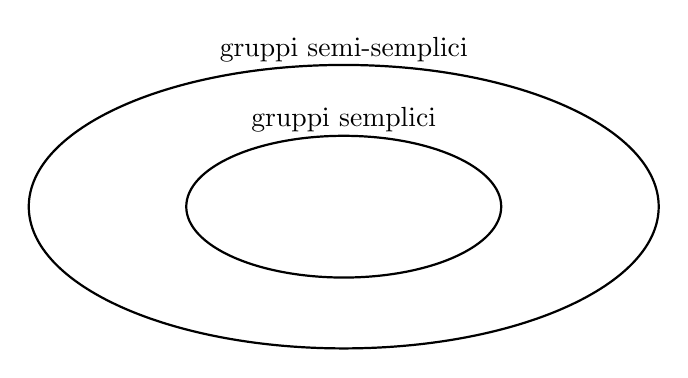
\begin{tikzpicture}
			\draw[fill=white, thick] (0, 2.5) ellipse (4cm and 1.8cm);
			\node[font=\normalsize] at (0, 4.5) {gruppi semi-semplici};
			\draw[fill=white, thick] (0, 2.5) ellipse (2cm and 0.9 cm);
			\node[font=\normalsize] at (0, 3.6) {gruppi semplici};
		\end{tikzpicture}
		\caption{Relazione insiemistica fra gruppi semplici e semi-semplici}
	\end{figure}
\end{remark}

Un altro oggetto molto importante, che possiamo definire a partire da un sottogruppo è il concetto di \emph{coset}
\begin{definition}[coset]
	Sia $(G, \circ)$ un gruppo,sia $g_i \in G$ e sia $H \subset G$ un sottogruppo, diremo che il coset sinistro di $H$ con \emph{rappresentante} $g_i$ è l'insieme degli elementi dati da
	\begin{equation}
		g_i \, \circ \, H. 
	\end{equation}
	L'insieme di tutti i coset è indicato con $G \, \backslash \, H$.
\end{definition}
\begin{remark}
	In pratica, stiamo vedendo gli elementi della forma $g_1 \circ h_1, g_1 \circ h_2, \ldots$ come il medesimo elemento, ovvero il coset di $H$ con rappresentante $g_i$: si potrebbe dare una definizione alternativa
	tramite relazione d'equivalenza dicendo che
	$$
		g_i \sim_H g_j \iff g_i^{-1} g_j \in H \iff g_j \in g_i H 
	$$
\end{remark}

\begin{remark}
	Si potrebbe definire anche il coset destro (noi sopra abbiamo fatto quello sinistro), come l'insieme degli elementi, fissato $g_i \in G$, della forma
	\begin{equation}
		H \, \circ \, g_i.
	\end{equation}
\end{remark}

Solitamente il coset non ha una struttura di gruppo rispetto a $\circ$, tuttavia si può mostrare che
\begin{prop} \label{prop:sott_inv_coset_grupp}
	Sia $(G, \circ)$ un gruppo e sia $H \subseteq G$ un sottogruppo invariante, allora $\equivcls{G}{H}$ è un gruppo rispetto a $\circ$
\end{prop} 
\begin{proof}
	Si ha infatti che presi $g_1 \circ H$ e $g_2 \circ H$ allora, essendo $H$ un sottogruppo invariante
	\begin{equation}
		g_1 \circ H \circ g_2 \circ H \stackrel{e = g_2 \circ g_2^{-1}}{=} g_1 \circ g_2 \circ \underbrace{g_2^{-1} H \circ g_2}_{\in H} H = g_1 \circ g_2 \circ H.
	\end{equation}
\end{proof}

\section{Omomorfismi}

Vogliamo analizzare, adesso, una classe di mappe fra gruppi molto importanti, che rispettano la struttura algebrica del gruppo. Prima di definire esplicitamente cosa siano, vediamo una situazione generale:
consideriamo due gruppi, che indichiamo con $(G_1, \circ_1), (G_2, \circ_2)$, e consideriamo una mappa $f: G_1 \to G_2$; in generale, si vede che, presi $a, b \in G_1$ abbiamo che
\begin{equation} \label{eq:strutt_alg}
	f(a \circ_1 b) \neq f(a) \circ_2 f(b).
\end{equation}
Questa proprietà di rispettare le operazioni fra i gruppi è ciò che si intende col rispettare la struttura algebrica del gruppo. Le mappe che rispettano la (\ref{eq:strutt_alg}) sono ciò che noi chiamiamo \textbf{omomorfismi}, di cui riportiamo la definizione formale qua sotto

\begin{definition}[omomorfismo]
	Siano $(G_1, \circ_1)$ e $(G_2, \circ_2)$ due gruppi (non necessariamente distinti), diremo che $f: G_1 \to G_2$ è un omomorfismo se
	\begin{equation}
		\forall a, b \in G_1, f(a \circ_1 b) = f(a) \circ_2 f(b).
	\end{equation}
\end{definition}

E' facile mostrare che
\begin{exercise}
	Siano $(G_1, \circ_1)$ e $(G_2, \circ_2)$ due gruppi e sia $f: G_1 \to G_2$ un omomorfismo, allora
	\begin{enumerate}[label=\protect\circled{\arabic*}]
		\item se $e_1$ è l'elemento neutro di $G_1$ e $e_2$ è l'elemento neutro di $G_2$, allora
		\begin{equation}
			f(e_1) = e_2,
		\end{equation}
		\item se $a \in G_1$, allora
		$$
			f(a^{-1}) = (f(a))^{-1}.
		$$
	\end{enumerate}
\end{exercise}
\begin{proof}
	Mostriamo la \circled{1}: è facile vedere, usando il fatto che $e_1 = e_1 \circ e_1$, che
	\begin{align}
		f(e_1) &= f(e_1 \, \circ_1 \, e_1) = f(e_1) \, \circ_2 \, f(e_1) \implies f(e_1) \, \circ_2 \, (f(e_1))^{-1} = f(e_1) \, \circ_2 \, f(e_1) \, \circ_2 \,(f(e_1))^{-1} \nonumber \\
		&\implies e_2 = f(e_1),
	\end{align}
	dove abbiamo usato il fatto che $G_2$ è comunque un gruppo, dunque ad ogni elemento esiste un suo inverso.
	Mostriamo la \circled{2}: 
	\begin{align}
		e_2 &= f(e_1) = f(a^{-1} \circ_1 a) = f(a^{-1}) \circ_2 f(a) \implies e_2 \circ_2 (f(a))^{-1} = f(a^{-1}) \circ_2 f(a) \circ_2 (f(a))^{-1} = \nonumber \\
			&= f(a^{-1}) \circ_2 e_2 = f(a^{-1}) \implies (f(a))^{-1} = f(a^{-1}).
	\end{align}
\end{proof}
Possiamo introdurre, similmente a come avevamo fatto per le applicazioni lineari fra spazi vettoriali, il kernel di un omomorfismo

\begin{definition}[kernel di un omomorfismo]
	Siano $(G_1, \circ_1)$ e $(G_2, \circ_2)$ due gruppi e sia $f: G_1 \to G_2$ un omorfismo fra i due. Allora definiamo kernel di $f$ come
	\begin{equation}
		\text{Ker}(f) = \{ g_1 \in G_1 : f(g_1) = e_2 \}.
	\end{equation}
\end{definition}
\begin{prop}
	$\text{Ker}(f)$ è un sottospazio invariante.
\end{prop}
\begin{proof}
\begin{align}
	&g^{-1} \circ_1 \text{Ker}(f) \circ_1 g \mapsto f(g^{-1}) \circ_2 f(\text{Ker}(f)) \circ_2 f(g) = (f(g))^{-1} \circ_2 e_2 \circ_2 f(g) = e_2 \implies \nonumber \\
	&\implies g^{-1} \circ (\text{Ker}(f)) \circ g \in \text{Ker}(f). 
\end{align}
\end{proof}
\begin{cor} \label{cor:g_ker_grupp}
	$\equivcls{G}{\, \text{Ker}(f)}$ è un gruppo rispetto a $\circ_G$.
\end{cor}
\begin{proof}
	E' sufficiente usare la \ref{prop:sott_inv_coset_grupp}.
\end{proof}

Tramite il kernel è possibile mostrare il seguente teorema

\begin{theorem}[Fondamentale degli omomorfismi]
    Siano $(G_1, \circ_1)$ e $(G_2, \circ_2)$ due gruppi e sia $f: G_1 \to G_2$ un omomorfismo surgettivo. Allora
    \begin{equation}
        G_1 / \text{Ker}(f) \cong \text{Im}(f)
    \end{equation}
\end{theorem}

% Per fare questa dimostrazione è necessario il seguente lemma:
% \begin{lemma} \label{lemma:eq_coset_ker}
% 	Sia $K$ il kernel di un omomorfismo $f: G_1 \to G_2$ con $(G_1, \circ_1)$ e $(G_2, \circ_2)$ due gruppi, allora $\forall a \in G_1$
% 	\begin{equation}
% 		aK = Ka.
% 	\end{equation}
% \end{lemma}
% \begin{proof}
% 	La dimostrazione verte nel far vedere che $aK \subseteq Ka$ e $Ka \subseteq aK$. Partiamo con la prima \\
% 	$\boxed{\subseteq}:$ sia $a \, \circ_1 \, k \in aK$, con $k \in K$, allora si ha che
% 	\begin{equation}
% 		f(a \, \circ_1 \, k \, \circ_1 \, a^{-1}) = f(a) \, \circ_2 \, f(k) \, \circ_2 \, f(a^{-1}) = f(a) \circ_2 (f(a))^{-1} = e_2,
% 	\end{equation}
% 	dunque $a \, \circ_1 k \, \circ_1 a^{-1} \in \text{Ker}(f),$ dunque $\exists k' \in K$ tale che
% 	\begin{equation}
% 		a \, \circ_1 k \, \circ_1 a^{-1} = k' \implies a \, \circ_1 k \, \circ_1 a^{-1} \, \circ_1 \, a = k' \, \circ_1 \, a,
% 	\end{equation}
% 	dunque $aK \subseteq Ka$. \\
% 	$\boxed{\supseteq}:$ sia $k \, \circ \, a \in Ka, k \in K$, allora si ha che
% 	\begin{equation}
% 		f(a^{-1} \, \circ_1 \, k \, \circ_1 \, a) = f(a^{-1}) \, \circ_2 \, f(k) \, \circ_2 \, f(a) = e_2,
% 	\end{equation}
% 	dunque $a^{-1} \, \circ_1 k \, \circ_1 \, a \in \text{Ker}(f)$, dunque $\exists k' \in K$ tale che
% 	\begin{equation}
% 		a^{-1} \, \circ_1 k \, \circ_1 \, a = k' \implies a \, \circ_1 a^{-1} \, \circ_1 k \, \circ_1 \, a = a \, \circ_1 \, k' \implies k \, \circ_1 \, a = a \, \circ_1 \, k',
% 	\end{equation}
% 	quindi $Ka \subseteq aK$.
% \end{proof}
\begin{proof}
    Sia $K = \text{Ker}(f)$. Si osserva che, se $a, a' \in G_1$ tali che $f(a) = f(a') = a^\star \in \text{Im}(f)$ allora
    \begin{equation}
        a^{-1} \, \circ_1 a' \stackrel{f}{\mapsto} f(a^{-1}) \, \circ_2 \, f(a') = (f(a))^{-1} \, \circ_2 \, f(a') = (a^\star)^{-1} \, \circ_2 \, a^\star = e_{2}, 
    \end{equation}
    dunque abbiamo che
    \begin{equation}
        a^{-1} \, \circ_1 \, a' \in K.
    \end{equation}
    Tuttavia si ha, a questo punto, che
    \begin{equation}
        a \, \circ_1 \, K = a \, \circ_1 \, (a^{-1} \, \circ_1 \, a') K = (a \, \circ_1 \, a^{-1}) \, \circ_1 \, a' K = a' \, \circ_1 \, K,
	\end{equation}
    dove abbiamo usato il fatto che se $k \in K \implies k \, \circ_1 \, K = K$, siccome $K$ ha la struttura di sottogruppo e $a^{-1} \, \circ_1 \, a' \in K$. 
    Dunque la mappa $\bar{f}$ che associa ad ogni coset di $K$ il valore di $f$ applicato all'elemento rappresentante del coset (ovvero $\bar{f}(aK) = f(a)$) è ben definita ed iniettiva. 
    
    Inoltre, la mappa è surgettiva su $\text{Im}(f)$: per definizione, $\forall b \in \text{Im}(f), \exists a \in G_1 : f(a) = b$, dunque $\exists aK \in G_1 / K : \bar{f}(aK) = b$.

    Infine, la mappa conserva l'operazione di gruppo: è sufficiente osservare che per la \ref{cor:g_ker_grupp} si ha che
    \begin{align}
        \bar{f}(aK \circ_1 bK) = \bar{f}(a \circ bK) = f(a \circ b) = f(a) \circ_2 f(b) = \bar{f}(aK) \circ_2 \bar{f}(bK).
    \end{align}
    Essendo biunivoca e un omomorfismo, $\bar{f}$ è un isomorfismo.
\end{proof}

Una particolare rilevante di isomorfismi è quello di \emph{automorfismo}, ovvero un isomorfismo da un gruppo in sé stesso. E' chiaro che l'insieme degli automorfismi sia un gruppo
rispetto all'operazione di composizione: sia $(G, \cdot)$ un gruppo e siano $g_1, g_2 : G \to G$ automorfismi, allora è chiaro che la funzione $g_1 \cdot g_2 : G \to G$ è ben definita e preso $a, b \in G$ abbiamo che
\begin{equation}
	(g_1 \circ g_2)(a \cdot b) = g_1(g_2(a \cdot b)) = g_1(g_2(a) \cdot g_2(b)) = g_1(g_2(a)) \cdot g_1(g_2(b)) = (g_1 \circ g_2)(a) \cdot (g_1 \circ g_2)(b),
\end{equation}
altrettanto chiaro è il fatto che, in generale, abbiamo
\begin{equation}
	g_1 \circ g_2 \neq g_2 \circ g_1.
\end{equation}
\begin{definition}[automorfismo e insieme degli automorfismi]
	Sia $(G, \circ)$ un gruppo e sia $f: G \to G$ un isomorfismo, diremo allora che $f$ è un automorfismo e indicheremo l'insieme degli automorfismi con $\text{Aut}(G)$. 
\end{definition}

Un automorfismo particolarmente rilevante è il concetto di \emph{automorfismo indotto}: sia $(G, \circ)$ un gruppo e sia $g \in G$ fissato, allora l'applicazione

\begin{equation}
	g \in G \mapsto h \, \circ \, g \,  \circ \, h^{-1} \in G,
\end{equation}

in quanto è suriettivo (preso $g \in G,$ allora abbiamo sicuramente che $h^{-1} \, \circ \, g \, \circ \, h$ è controimmagine di $g$) ed è iniettivo (siccome se $f(g_1) = f(g_2) \implies 
h \, \circ \, g_1 \, \circ \, h^{-1} = h \, \circ \, g_2 \, \circ \, h^{-1} \implies g_1 \, \circ \, h^{-1} = g_2 \, \circ \, h^{-1} \implies g_1 = g_2$) e il fatto che sia un omomorfismo deriva dal fatto che

\begin{equation}
	g_1 \, \circ \, g_2 \mapsto h \, \circ \, g_1 \, \circ g_2 \, \circ \, h^{-1} = h \, \circ \, g_1 \, \circ \, h^{-1} \, \circ \, h \, \circ \, g_2 \, \circ \, h^{-1} = f(g_1) \, \circ \, f(g_2). 
\end{equation}
